\documentclass[aspectratio=169]{beamer}
\usepackage{tabularx}
% --------------------------------------------------
% Opções para "aspectratio"
% 43 ou 54: Formatos 4:3 ou 5:4 tradicionais para telas antigas
% 169, 1610 ou 189: Formatos 16:9, 16:10 ou 18:9 widescrenn telas mais modernas
% --------------------------------------------------
\usepackage{ifslides2024} % Tema (não remover)
\usepackage{lipsum}       % Gerador de texto dummy
\usepackage{csquotes}
\usepackage[utf8]{inputenc}

\addbibresource{referencias.bib} % Referências
% Dados da Apresentação
\vspace*{0.2cm}
\titulo{ ANÁLISE COMPARATIVA ENTRE ALGORITMOS DE PREDIÇÃO DE PREÇO PARA O BITCOIN}
\subtitulo{Trabalho de conclusão de curso}
\autor{Mickael Osvaldo de Oliveira}
\email{mickaelosvaldo1999@gmail.com}
\info{% Informações adicionais (opcional)
  Bacharelado em Engenharia de Computação \\%
  \textbf{Orientador:} Prof. Dr. Ciniro Aparecido Leite Nametala \\% 
}
\campus{Bambuí}
\data{2025}

\begin{document}

% Página inicial
\begin{frame}[plain, fragile]
  \titlepage
\end{frame}

% ------------------------------------------------------------

% Sumário
\begin{frame}[fragile]{Sumário}
  \tableofcontents
\end{frame}

% ------------------------------------------------------------

\section{Introdução}

\begin{frame}[plain,fragile,t] \frametitle{Introdução}
	\begin{center}
	\end{center}
\end{frame}

% ------------------------------------------------------------

\subsection{Contextualização}

\begin{frame}[fragile] \frametitle{Introdução -- Contextualização}
	\begin{itemize} \itemsep1em
	\item 	A predição de preços em ativos financeiros teve sua origem atribuída a \textcite{Bachelier}, na teoria conhecida como \textit{Random Walks} \cite{Fama1965,Fama,Courtault};
		
	\item 	Desde então, diversos métodos foram empregados com esse fim, destacando-se a análise técnica, fundamentalista e a utilização de modelos estatísticos como o ARIMA \cite{Ariyo} ou aprendizado de máquina \cite{Fer};
		
	\item 	Com advento da \textit{Blockchain} e \textit{Bitcoin} por \cite{Nakamoto}, um novo mercado de ativos descentralizados surgiu, trazendo consigo a necessidade de novas abordagens de predição de preços \cite{Zhang}.
	\end{itemize} \itemsep1em
\end{frame}

% ------------------------------------------------------------

\subsection{Objetivos}

\begin{frame}[fragile] \frametitle{Introdução -- Objetivos}
\begin{block}{Objetivo Geral}
  Analisar por meio comparativo o desempenho de algoritmos de predição de
preço no contexto do \textit{Bitcoin}.
\end{block}
\vskip1em
\begin{block}{Objetivos Específicos} 
  \begin{enumerate}
    \item Desenvolver a estrutura computacional necessária para selecionar, implementar
    e realizar previsões por meio de ferramentas tecnológicas adequadas;
    
    \item Validar de algoritmos de redes neurais e compará-los, frente aos Benchmarks de interesse, a fim de determinar qual tem melhor desempenho;

    \item Explorar de possíveis variações em métodos conhecidos, visando adaptá-los a um novo cenário;
  
    \item Analisar se esses métodos de predição são rentáveis em uma base de dados real.

  \end{enumerate}
\end{block}
\end{frame}

% ------------------------------------------------------------

\subsection{Justificativa}

\begin{frame}[fragile] \frametitle{Introdução -- Justificativa}
	\begin{itemize} \itemsep1em

    \item Os criptoativos tem se tornado uma alternativa ao mercado financeiro tradicional, principalmente devido a sua volatilidade, tem sido adotado como ativo de alto risco \cite{Sousa};
			
		\item Esta pesquisa busca comparar algorítmos de predição de preços, sejam estatísticos ou de aprendizado de máquina, a fim de avaliar seu desempenho em uma base de dados real;
			
		\item As tecnologias convergem para um cenário onde a análise de dados é cada vez mais importante, a inteligência artificial e a rede distribuída são a parte central da Web3;
		
    \item Os modelos utilizados serão o ARIMA, LSTM, BiLSTM e GRU. Em que todas as implementações estarão públicas no \textit{GitHub}.
		
    \end{itemize}
\end{frame}

% ------------------------------------------------------------

\section{Fundamentação Teórica}

\begin{frame}[plain,fragile,t] \frametitle{Fundamentação Teórica}
\end{frame}

% ------------------------------------------------------------



% ------------------------------------------------------------

\subsection{Fundamentos conceituais}

\begin{frame}[fragile] \frametitle{Fundamentação Teórica -- Fundamentos conceituais}
	\begin{itemize} \itemsep1em
		\item A ideia de Ativos Digitais descentralizados baseados em criptografia, ou criptomoedas, foi marcada por inúmeras tentativs anteriores, mas só foi implementada como advento da \textit{Blockchain} por \textcite{Nakamoto} \cite{Moi};
		\item O ARIMA (\textit{Autoregressive Integrated Moving Average}) tem suas raízes na econometria e na estatística. Sua história remonta ao trabalho pioneiro de \textcite{Box};
		\item A teoria de Redes Neurais Artificiais teve início com os estudos de \textcite{Rosenblatt}, evoluiu com \textcite{Rumelhart}. Atualmente, é associada ao aprendizado profundo proposto por \textcite{Good}.
	\end{itemize}
\end{frame}

\begin{frame}[fragile] 
    \frametitle{Fundamentação Teórica -- Bitcoin}
    \begin{itemize}
		\item O Bitcoin é definido como um dinheiro eletrônico negociado diretamente entre pares, sem passar por uma instituição financeira \cite{Nakamoto};
		\item \textcite{Yuan} descrevem a \textit{Blockchain} como um registro compartilhado distribuído, onde a confiança mútua entre as partes é estabelecida por algoritmos matemáticos.
	\end{itemize}

	\begin{columns}[c]
		\begin{column}{1\linewidth}
			\begin{figure}
				\fbox{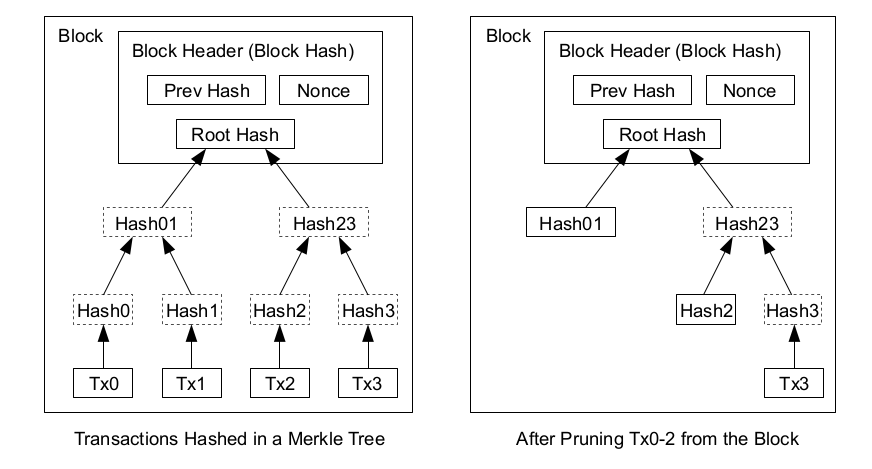
\includegraphics[scale=0.15]{figuras/blockchain.png}}
				\label{fig:blockchain}
			\end{figure}

			\begin{block}{Figura 1 - Transações na \textit{Blockchain.}}
				Figura que contém a árvore de Markle inserida na \textit{Blockchain.} \newline Fonte: \cite{Nakamoto}.    
			\end{block}
		\end{column}
	\end{columns}
\end{frame}


\subsection{Modelos}

\begin{frame}[fragile] 
    \frametitle{Fundamentação Teórica -- ARIMA}
    \begin{itemize}
		\item Abordagem sistemática para identificar, estimar e diagnosticar modelos de séries temporais, conhecida como metodologia Box-Jenkins \cite{Arima};
		\item Atribui-se a cada uma das componentes do modelos as siglas \textit{p}, \textit{d} e \textit{q} representado o ajuste na série. O parâmetro \textit{p} é a ordem do modelo AR, \textit{d} é o grau de diferenciação (I) e \textit{q} é a ordem do modelo MA.
	\end{itemize}
\end{frame}

\begin{frame}[fragile] 
    \frametitle{Fundamentação Teórica -- Redes neurais artificiais}
    \begin{columns}[c]
		\begin{column}{1\linewidth}
			\begin{figure}
				\fbox{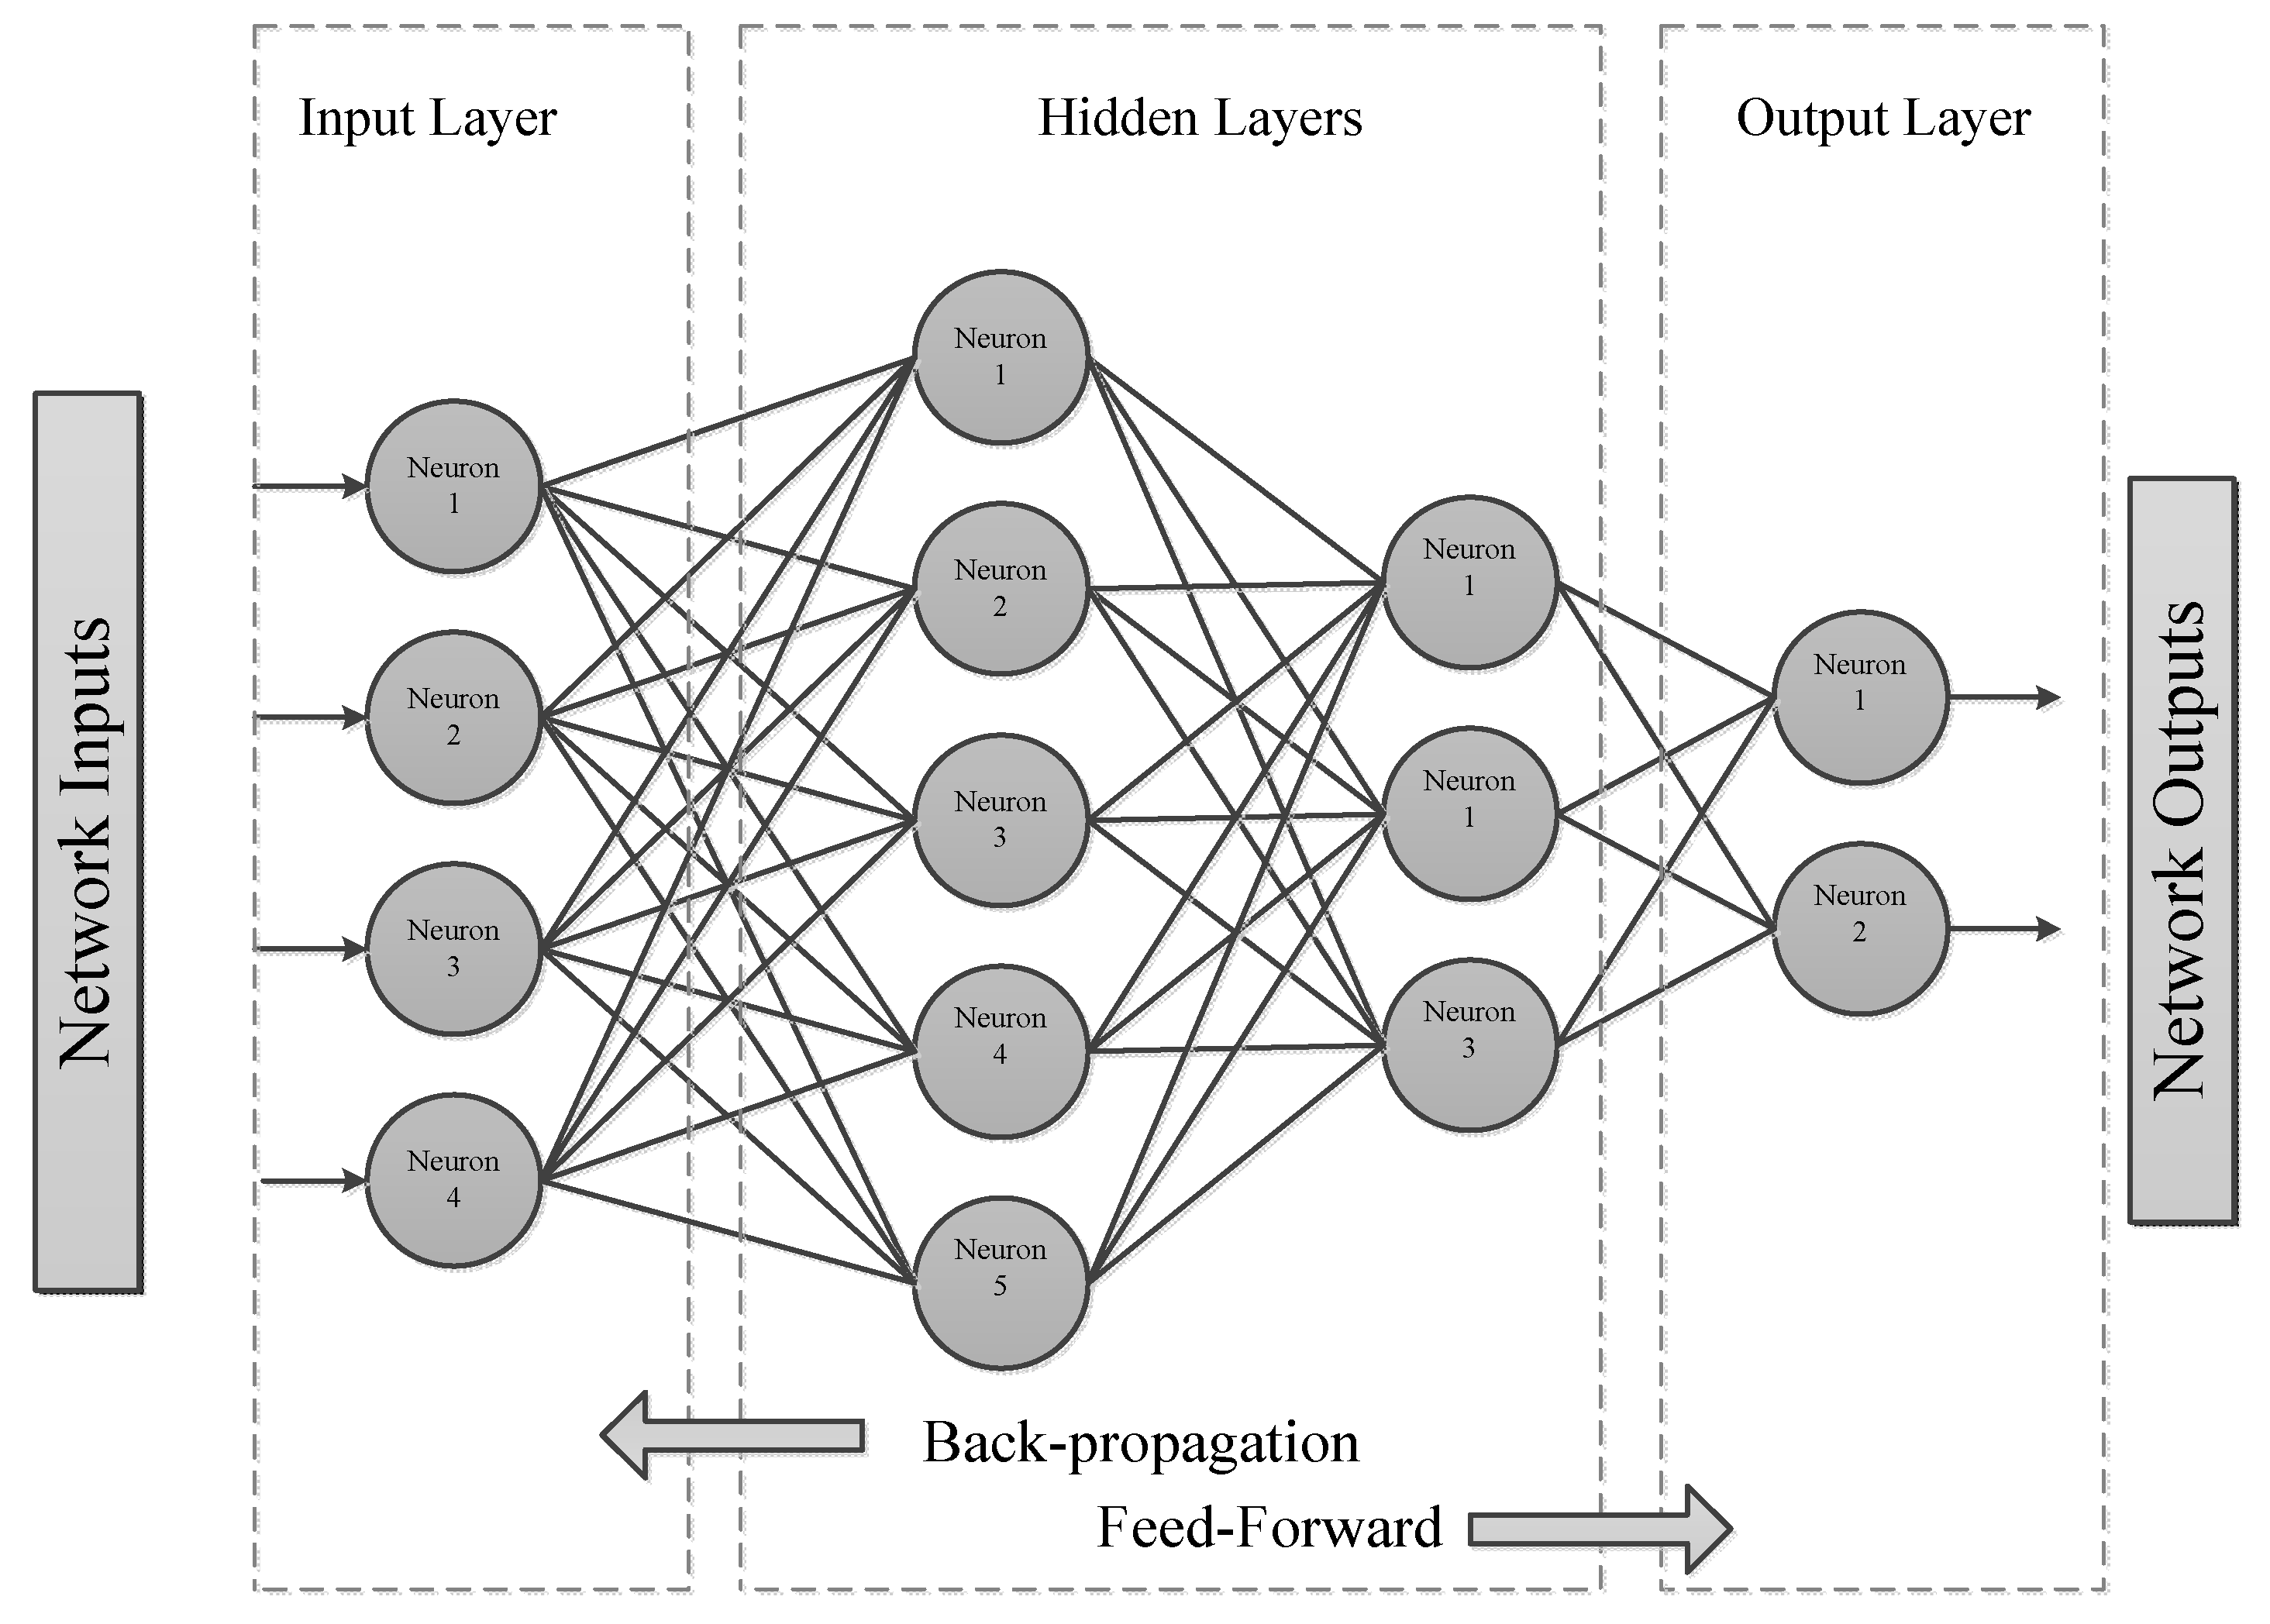
\includegraphics[scale=0.065]{figuras/mlp.png}}
				\label{fig:mlp}
			\end{figure}

			\begin{block}{ Figura 2 - \textit{Multilayer Perceptron (MLP)}}
				Figura contendo uma MLP com duas camadas escondidas. \newline Fonte: \cite{multilayer}.    
			\end{block}
		\end{column}
	\end{columns}
\end{frame}

\begin{frame}[fragile] 
    \frametitle{Fundamentação Teórica -- \textit{Long Short-Term Memory (LSTM)}}
    \begin{columns}[c]
		\begin{column}{1\linewidth}
			\begin{figure}
				\fbox{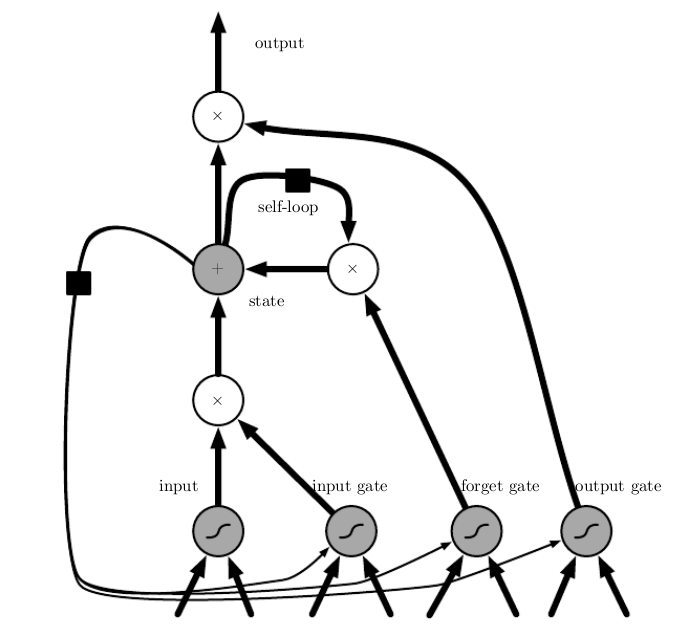
\includegraphics[scale=0.2]{figuras/lstm.png}}
				\label{fig:lstmStr}
			\end{figure}

			\begin{block}{ Figura 3 - Estrutura de uma LSTM}
				Figura que contêm a estrutura básica da LSTM. \newline Fonte: \cite{graves}.    
			\end{block}
		\end{column}
	\end{columns}
\end{frame}

\begin{frame}[fragile] 
    \frametitle{Fundamentação Teórica -- \textit{Bidirecional LSTM (BiLSTM)}}
	\begin{itemize}
		\item Processa a sequência em duas direções, do futuro para o passado e do passado para o futuro;
		\item Melhora o desempenho em tarefas que exigem a interpretação completa da sequência do \textit{input};
		\item Ao final, as saídas são concatenadas e passadas para a camada seguinte.
	\end{itemize}
\end{frame}

\begin{frame}[fragile] 
    \frametitle{Fundamentação Teórica -- \textit{Gated Recurrent Unit (GRU)}}
    \begin{columns}[c]
		\begin{column}{1\linewidth}
			\begin{figure}
				\fbox{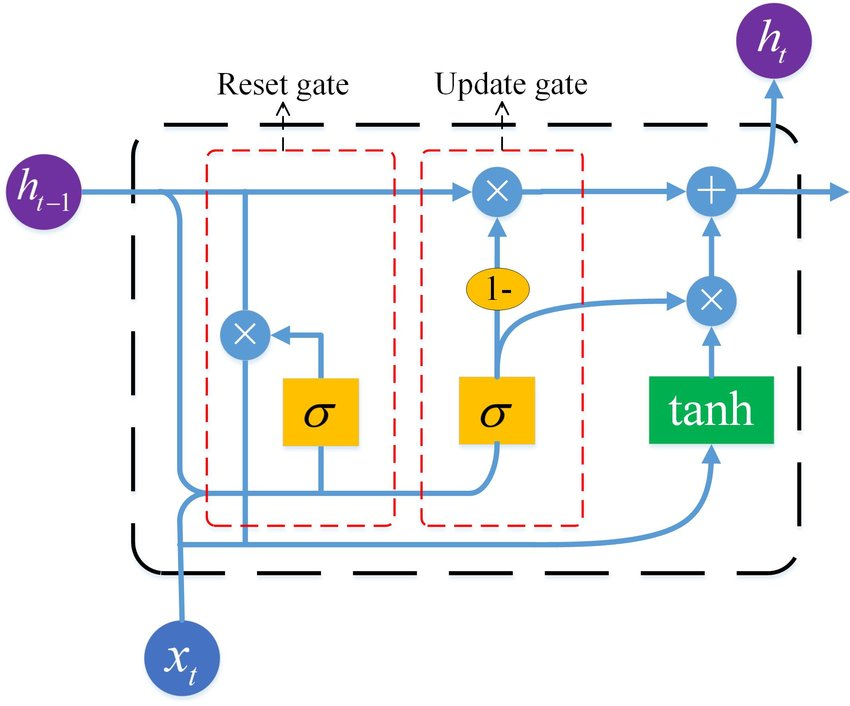
\includegraphics[scale=0.7]{figuras/gru.png}}
				\label{fig:gruStr}
			\end{figure}

			\begin{block}{Figura 4 - Estrutura de uma GRU}
				Figura que contêm o diagrama de uma unidade de GRU. \newline Fonte: \cite{gru-image}.    
			\end{block}
		\end{column}
	\end{columns}
\end{frame}



\subsection{Revisão Bibliográfica}
\begin{frame}[fragile] 
    \frametitle{Fundamentação Teórica -- Revisão Bibliográfica}
    \begin{columns}[c]
		\begin{column}{1\linewidth}
			\begin{figure}
				\fbox{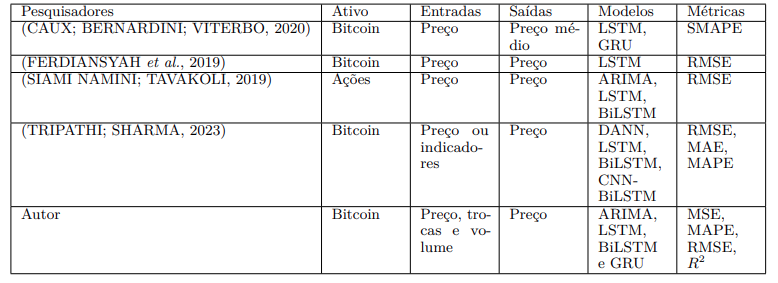
\includegraphics[scale=0.3]{figuras/estudos.png}}
				\label{fig:estudos}
			\end{figure}

			\begin{block}{Tabela 1 - Estudos similares}
				Tabela que enumera os principais estudos relacionados ao tema. \newline Fonte: Próprio autor.    
			\end{block}
		\end{column}
	\end{columns}
\end{frame}

% ------------------------------------------------------------

\section{Metodologia}

\begin{frame}[plain,fragile,t] \frametitle{Metodologia}
\end{frame}

% ------------------------------------------------------------

\subsection{Classificação da pesquisa}

\begin{frame}[fragile] \frametitle{Metodologia -- Classificação da pesquisa}
	\begin{itemize}
		\item Pode-se dizer, segundo a abordagem de \textcite{pesquisa}, que a pesquisa adota uma abordagem quantitativa e experimental;
		
		\item A natureza aplicada do
    estudo busca não apenas compreender as nuances de cada algoritmo, mas também oferecer
    insights para a seleção e implementação dos mais eficazes;
		
		\item A metodologia descritiva permite
    uma análise detalhada dos resultados obtidos, destacando as diferenças significativas entre
    os modelos avaliados.
	\end{itemize}
\end{frame}

% ------------------------------------------------------------

\subsection{Solução proposta}

\begin{frame}[fragile] \frametitle{Metodologia -- Solução proposta}
	\begin{itemize}
		\item Utilizou-se a linguagem de programação \textit{Python} e bibliotecas para extrair, tratar e analisar os dados os presentes na \textit{Binance};
		
		\item O \textit{Dataset} obtido conta com 26.304 amostras com o histórico de preços do Bitcoin em intervalos de 15 minutos, com dados como trocas, volume e preço entre Janeiro e Outubro de 2020;
		\item Para treinar as redes neurais foi utilizado um janelamento de 24 amostras (6 horas) enquanto o ARIMA foi parametrizado com o auto ARIMA.
	\end{itemize}
\end{frame}


\begin{frame}[fragile]
	\frametitle{Metodologia -- Solução proposta}
		\begin{columns}[c]
			\begin{column}{1\linewidth}
				\begin{figure}
					\fbox{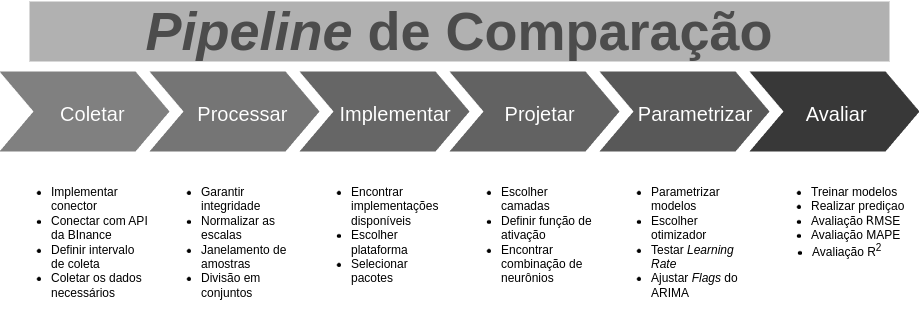
\includegraphics[scale=0.35]{figuras/proposta.png}}
					\label{fig:proposta}
				\end{figure}

				\begin{block}{Figura 5 - Fluxo de comparação dos algoritmos}
					Figura ilustrativa dos passos para a comparação dos algoritmos. \newline Fonte: Próprio autor.    
				\end{block}
			\end{column}
		\end{columns}
	\end{frame}

% ------------------------------------------------------------

\section{Resultados}

\begin{frame}[plain,fragile,t] \frametitle{Resultados}
\end{frame}

\begin{frame}[fragile]
	\frametitle{Resultados - LSTM}

	\begin{itemize} 
		\item O gráfico obtido após a aplicação do LSTM foi:
	\end{itemize}

		\begin{columns}[c]
			\begin{column}{1\linewidth}
				\begin{figure}
					\fbox{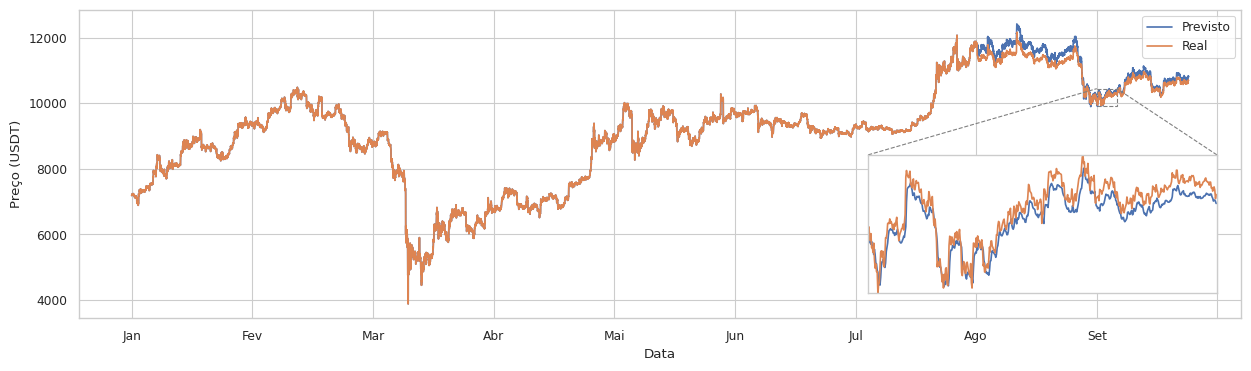
\includegraphics[scale=0.25]{figuras/lstmOutput.png}}
					\label{fig:lstm}
				\end{figure}

				\begin{block}{Gráfico de saída do LSTM}
					Gráfico que retrata a comparação do previsto no LSTM (Azul) com o real (Laranja). \newline Fonte: Próprio autor.    
				\end{block}
			\end{column}
		\end{columns}
	\end{frame}

\begin{frame}[fragile]
	\frametitle{Resultados - BiLSTM}

	\begin{itemize} 
		\item O gráfico obtido após a aplicação do BiLSTM foi:
	\end{itemize}

		\begin{columns}[c]
			\begin{column}{1\linewidth}
				\begin{figure}
					\fbox{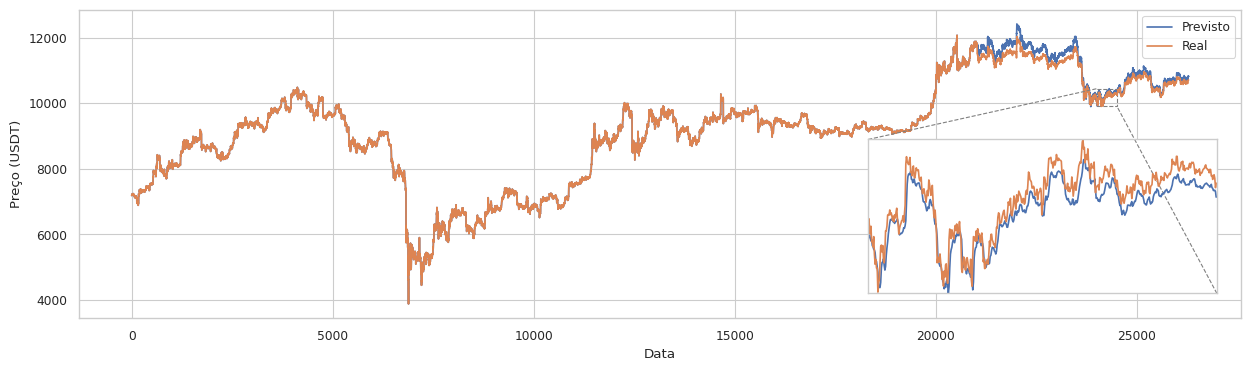
\includegraphics[scale=0.25]{figuras/bilstmOutput.png}}
					\label{fig:bilstm}
				\end{figure}

				\begin{block}{Gráfico 1 - Saída do BiLSTM}
					Gráfico que retrata a comparação do previsto no BiLSTM (Azul) com o real (Laranja). \newline Fonte: Próprio autor.    
				\end{block}
			\end{column}
		\end{columns}
	\end{frame}


	\begin{frame}[fragile]
		\frametitle{Resultados - GRU}
	
		\begin{itemize} 
			\item O gráfico obtido após a aplicação do GRU foi:
		\end{itemize}
	
			\begin{columns}[c]
				\begin{column}{1\linewidth}
					\begin{figure}
						\fbox{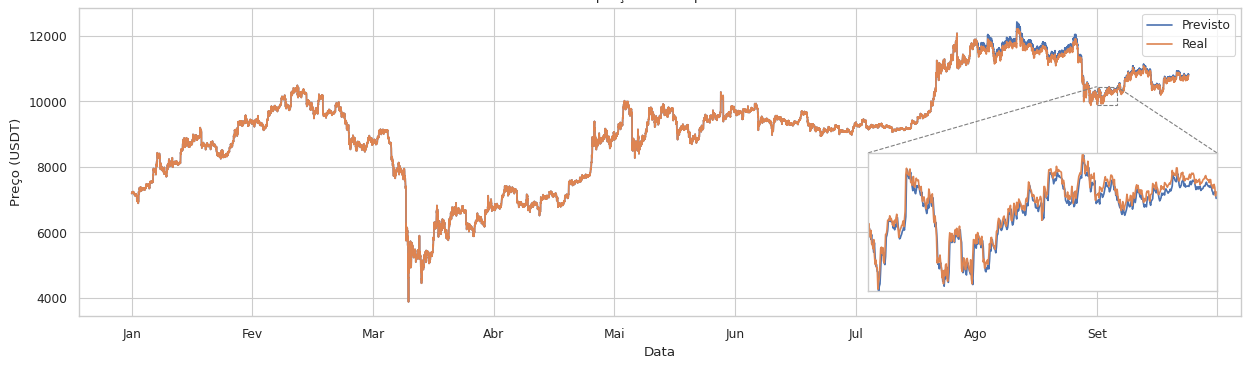
\includegraphics[scale=0.25]{figuras/gruOutput.png}}
						\label{fig:gru}
					\end{figure}
	
					\begin{block}{Gráfico 2 - Saída do GRU}
						Gráfico que retrata a comparação do previsto no GRU (Azul) com o real (Laranja). \newline Fonte: Próprio autor.    
					\end{block}
				\end{column}
			\end{columns}
		\end{frame}

	
		\begin{frame}[fragile]
			\frametitle{Resultados - ARIMA}
		
			\begin{itemize} 
				\item O gráfico obtido após a aplicação do ARIMA foi:
			\end{itemize}
		
				\begin{columns}[c]
					\begin{column}{1\linewidth}
						\begin{figure}
							\fbox{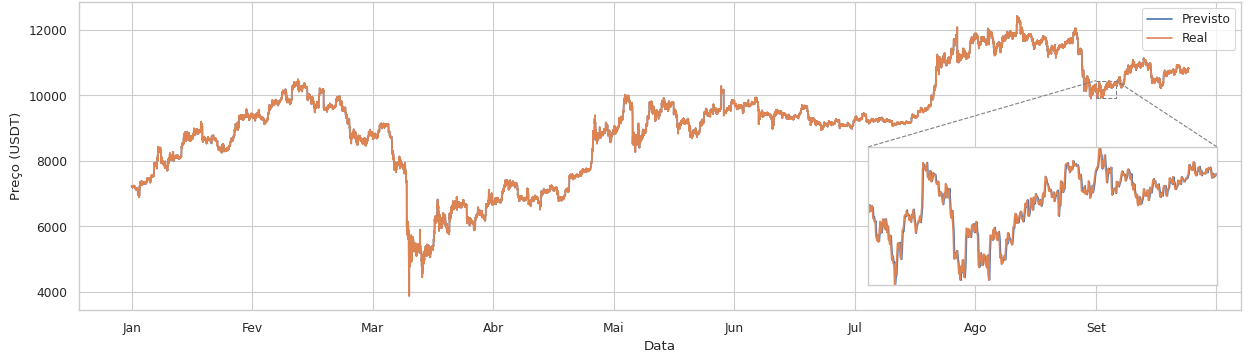
\includegraphics[scale=0.25]{figuras/arimaOutput.png}}
							\label{fig:arima}
						\end{figure}
		
						\begin{block}{Gráfico 3 - Saída do ARIMA}
							Gráfico que retrata a comparação do previsto no ARIMA (Azul) com o real (Laranja). \newline Fonte: Próprio autor.    
						\end{block}
					\end{column}
				\end{columns}
			\end{frame}

\begin{frame}[fragile] \frametitle{Resultados - Classificação dos modelos}
	\begin{itemize} 
		\item Os resultados finais após os testes dos modelos foram:
	\end{itemize}
	\begin{columns}[c]
		\begin{column}{0.6\linewidth} % Reduz a largura da coluna para evitar overflow
			\begin{table}[!htb]
				\resizebox{\linewidth}{!}{ % Ajusta a tabela automaticamente
				\begin{tabular}{|c|c|c|c|c|}
				\hline
				Posição & Nome & RMSE & $R^2$ & MAPE \\ \hline
				1° & ARIMA   & 28,9699      & 0,9989           & 0,0016             \\ \hline
				2° & GRU   & 86,1828      & 0,9799             & 0,0064             \\ \hline
				3° & LSTM   & 193.5493      &  0,8990           & 0,0145                \\ \hline
				4° & BiLSTM   & 207,2416    & 0,8842            & 0,0153           \\ \hline
				\end{tabular}
				}
			\end{table}
		\end{column}
	\end{columns}
	\begin{block}{Tabela 2 - Resultados obtidos}
		Tabela contendo os erros e classificação de cada modelo no \textit{Dataset} utilizado. \newline Fonte: Próprio autor.    
	\end{block}
\end{frame}

\section{Conclusões}

\begin{frame}[plain,fragile,t] \frametitle{Conclusões}
	
\end{frame}

% ------------------------------------------------------------

\begin{frame}[fragile] \frametitle{Conclusões}
	\begin{itemize}
		\item Foram exploradas diferentes métodos para a previsão do preço do Bitcoin em intervalos de 15 minutos, comparando métodos estatísticos e redes neurais;
		
		\item O modelo ARIMA obteve os melhores resultados no contexto, superando ligeiramente os modelos de rede neural ao apresentar previsões mais consistentes;
		\item Como continuidade para este trabalho, sugere-se a investigação de abordagens
		híbridas. Além disso, é possível expandir os testes para outros períodos e ativos financeiros.
	\end{itemize}
\end{frame}

\section{Referências}

\begin{frame}[allowframebreaks] 
\frametitle{Referências}
  \printbibliography 
\end{frame}

\begin{frame}[fragile,plain] \frametitle{Obrigado}
\begin{center}
 \vspace*{2em}

 Favor enviar as sugestões e os pedidos de correção para:

 mickaelosvaldo1999@gmail.com 
 
 ciniro.nametala@ifmg.edu.br.

 \vspace*{2em}
 
\includegraphics[width=1.5cm]{logoif}
\end{center}
\end{frame}

\end{document}
